\documentclass[9pt, twocolumn]{extarticle}

%%% Using extarticle instead of the standard article class to allow 8pt font size
%%% Title and author fields are manually resized (e.g., \Huge, \large) for better fitting
%%% \vspace*{-\topskip} is applied in \maketitle to remove the extra top margin above the title

\usepackage{graphicx}
\graphicspath{{../figs/}}
\usepackage[a4paper, margin=1.5cm, bottom=2.5cm]{geometry}
\usepackage{float}
\usepackage{subfig}
\usepackage{caption}
\usepackage{tabularx}
\usepackage{booktabs}
\usepackage{amsmath}
\usepackage{stfloats}
\usepackage{titlesec}
\usepackage{setspace}
\usepackage{xcolor}
\definecolor{UIUC_orange}{HTML}{FF5F05}
\usepackage[colorlinks=true,
            linkcolor=UIUC_orange,
            urlcolor=UIUC_orange,
            citecolor=UIUC_orange]{hyperref}
\usepackage[
  backend=biber,
  style=numeric,          % numbered refs
  citestyle=numeric-comp, % [1-3] compression
  sorting=none            % order of citation
  ]{biblatex}
  \addbibresource{references.bib}

\newcommand{\mystretch}{1.2}
\newcommand{\myfigmargin}{4pt}


\setlength{\textfloatsep}{\myfigmargin}    % text ↔ top/bottom floats
\setlength{\intextsep}{\myfigmargin}       % text ↔ here-placed floats ([h])
\setlength{\floatsep}{\myfigmargin}        % between floats
\setlength{\dbltextfloatsep}{\myfigmargin} % two-column floats (figure*)
\setlength{\dblfloatsep}{\myfigmargin}


\captionsetup[figure]{belowskip=0pt, skip=4pt, labelfont=bf, justification=justified, singlelinecheck=false, font={stretch=\mystretch}}
\captionsetup[subfloat]{labelfont=normalfont, justification=centering, singlelinecheck=false, farskip=4pt,captionskip=0pt, font={stretch=\mystretch}}
% \captionsetup[figure]{belowskip=-14pt, font={stretch=\mystretch}}
\captionsetup[subfloat]{belowskip=-14pt, font={stretch=\mystretch}}
\captionsetup[table]{labelfont=bf, justification=justified, singlelinecheck=false, skip=2pt, farskip=0pt, captionskip=0pt, belowskip=0pt, font={stretch=\mystretch}}
  
\renewcommand{\baselinestretch}{\mystretch} % 1.2x line spacing
  
\setlength{\columnsep}{0.5cm}
  
\makeatletter
\renewcommand\section{\@startsection{section}{1}{0pt}%
  {0.8ex plus 0.5ex minus 0.2ex}%
  {0.5ex}%
  {\normalfont\Large\bfseries}}
\makeatother


\makeatletter
\renewcommand{\maketitle}{\bgroup\setlength{\parindent}{0pt}
\vspace*{-\topskip}% remove the top margin above title
\begin{flushleft}
  \huge\textbf{\@title}

  \vspace{0.20cm}

  \normalsize\@author \hfill \normalsize\@date

  \vspace{0.25cm}\hrule\vspace{0.25cm}
\end{flushleft}
\egroup}
\makeatother


\title{Rainfall-Soil Moisture Event Responses near Baton Rouge, Louisiana}
\author{%
  % Ali Haghighi\thanks{University of Tehran, \href{mailto:ahaghighi@ut.ac.ir}{ahaghighi@ut.ac.ir}}%
  % Afshin Ashrafzadeh\thanks{University of Tehran, \href{mailto:a.ashrafzadeh@ut.ac.ir}{a.ashrafzadeh@ut.ac.ir}}%
  \large Ali Haghighi \normalsize{(ahaghighi@ut.ac.ir)}\large, Afshin Ashrafzadeh \normalsize{(a.ashrafzadeh@ut.ac.ir)}
}
\date{\large \today}



\begin{document}

\twocolumn[
  \begin{@twocolumnfalse}
    \maketitle
  \end{@twocolumnfalse}
]

% \makeatletter
% \@thanks
% \makeatother

\section{Introduction}

Rainfall governs soil moisture variability and drives hydrological processes from infiltration to contaminant transport. This study provides a concise, high-level analysis of event-scale rainfall–soil moisture interactions near Baton Rouge, Louisiana, during 2022–2024. We identify individual rainfall events, quantify their soil moisture responses, and highlight the interplay among pre-event soil moisture, post-event soil moisture, soil moisture change ($\Delta \theta$), and event precipitation. The framework has potential for future expansion to incorporate nitrate leaching and surface-subsurface contamination analysis.

\noindent\textbf{Resources: }
Codes and processed data (spatially and temporally subsampled; easy-to-use CSV) are available on \href{https://github.com/Alioax/rainfall-soil-moisture/}{GitHub repository}. 
My personal website and other projects can be found at \href{https://ciarel.com}{Ciarel.com}.

\begin{figure}[!b] % htbp
  \centering
  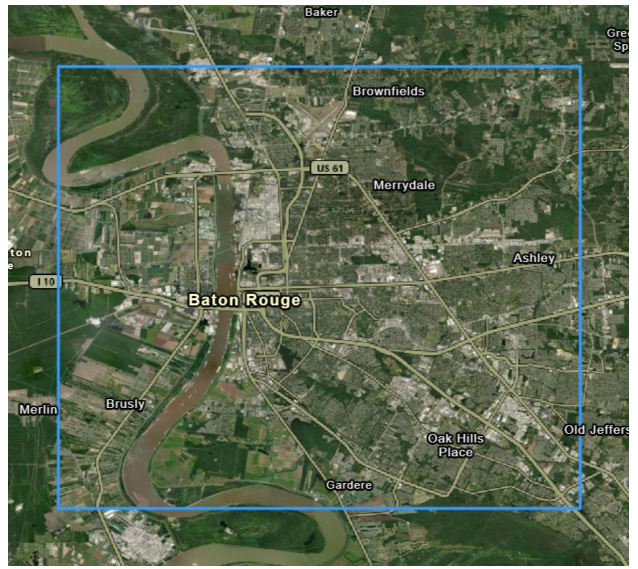
\includegraphics[width=0.95\columnwidth]{map}
  \caption{Study area near Baton Rouge, Louisiana. The analysis domain (25 $\times$ 25 km box) is outlined and overlain on regional context.}
  \label{fig:map}
\end{figure}

\section{Study Area and Data}

The analysis domain is a 25~$\times$~25~km box surrounding Baton Rouge, Louisiana (SW: 30.34,~-91.28; NE: 30.56,~-91.02), as shown in Fig.~\ref{fig:map}. This bounding box was chosen to capture regional hydroclimatic variability while maintaining a tractable spatial scale for event-based soil moisture analysis. Both precipitation and soil moisture datasets were subsetted spatially to this domain and temporally to the period 2022--2024.

Soil moisture conditions were obtained from the NASA Soil Moisture Active Passive (SMAP) mission, using the Enhanced Level-3 Radiometer Global Daily product (9~km resolution), which provides surface soil moisture retrievals representative of the top $\sim$5~cm of soil \cite{smap}. Precipitation data were obtained from the Global Precipitation Measurement (GPM) mission's Integrated Multi-satellite Retrievals (IMERG) Final Run product, available at 0.1$^{\circ}$ spatial and daily temporal resolution \cite{imergdp}.

Together, SMAP and IMERG provide harmonized, global-scale, open-access satellite observations suitable for characterizing - moisture interactions in regions such as Baton Rouge, where high-frequency precipitation events and strong seasonal cycles affect vadose-zone hydrology.


\section{Methods}

Rainfall events were defined from daily precipitation \(P_t\). A wet day is \(P_t \geq 1\) mm, and an event is a sequence of wet days that (i) starts after a dry day, and (ii) includes a burst of at least 5 mm on the first or second day. For an event with start \(s\) and end \(e\), total rainfall and duration are  
\[
R = \sum_{t=s}^{e} P_t, 
\qquad 
D = e - s + 1.
\]

Pre-event soil moisture is the mean of the three days before the event, but if these overlap with the previous event, we trim them. Let \(A\) denote this window and \(\theta_A\) its average. The post-event response window is
\[
B = \big[s,\; \min(e+3,\; s_{\mathrm{next}}-1)\big],
\qquad 
\theta_{\max} = \max_{t \in B} \theta_t .
\]

The main metric is the soil moisture increment  
\[
\Delta \theta = \theta_{\max} - \theta_A .
\]

We also compute a nominal lag between pre-event soil moisture and response times. However, we do not analyze it further because SMAP provides only surface soil moisture (\(\sim\)0--5 cm) at daily resolution. With no information from deeper layers, infiltration timing and true lags cannot be extracted reliably. If multi-depth soil measurements were available, lag analysis would be a valuable extension.  

\section{Results}

\textbf{Hydroclimatic context.} Monthly precipitation and domain-mean soil moisture (Fig.~\ref{fig:monthly_precip_sm}) track each other closely, with wetter months yielding higher soil moisture. Peaks occur at the end of winter and early spring, reflecting cumulative cool-season rainfall and low evaporative demand.

\textbf{Rainfall events.} Event characteristics are shown in Fig.~\ref{fig:rain_events}. The median event produced 25~mm over 2~days. High-depth, long-duration outliers (above the 75th percentile in both) occurred mainly in summer. Seasonal counts were Winter~31, Spring~31, Summer~29, and Autumn~23.

\textbf{Soil moisture responses.} For each rainfall event, the soil moisture increment ($\Delta \theta$) was calculated. Fig.~\ref{fig:sample_events} shows representative cases, highlighting how soil moisture responds to multi-day storms while smaller events are sometimes undetected by the event definition. Aggregated results across all events are summarized in Fig.~\ref{fig:dt_events}. The panels illustrate how $\Delta \theta$, pre-event soil moisture, post-event soil moisture, and event precipitation interact. A clear saturation boundary emerges: high pre-event moisture constrains additional gains, whereas drier conditions allow increases up to 18\%. Seasonal clustering reflects this—winter and spring events occur near saturation, while summer and autumn cover a broader, drier range. Looking at the distributions of pre- and post-event soil moisture (top boxplots), a clear shift toward higher values is evident: while the overall range remains similar, the distribution skews toward the upper bound ($\approx$45\%), and the post-event median even exceeds the pre-event 75th percentile.

\section{Future Research}

Future research could extend this event-based framework by incorporating nitrate, deeper soil moisture, and aquifer data into a fully integrated modeling approach, as in \textcite{Fahs2025}. This would allow exploration of contamination transport and aquifer interaction in addition to rainfall-driven infiltration responses. Such analysis could also be highly valuable in regions with scarce rainfall, where farmers must rely on rainfall-soil moisture assessments and predictions for decision-making \cite{haghighi}.

\begin{figure}[!h] % htbp
  \centering
  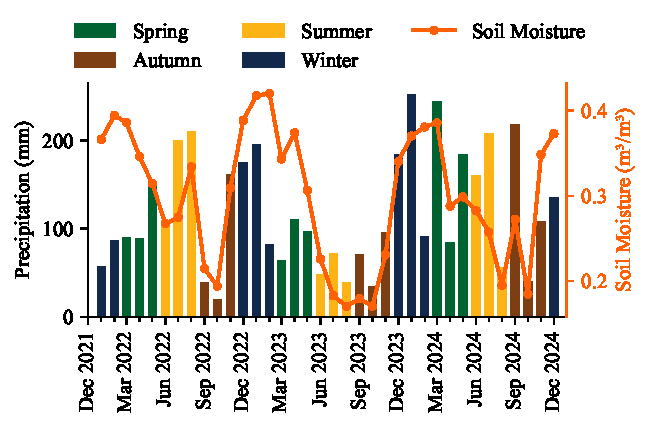
\includegraphics[width=1\columnwidth]{monthly_precip_sm}
  \caption{Monthly precipitation totals and averaged soil moisture from 2022-2024.}
  \label{fig:monthly_precip_sm}
\end{figure}

\begin{figure}[!h] % htbp
  \centering
  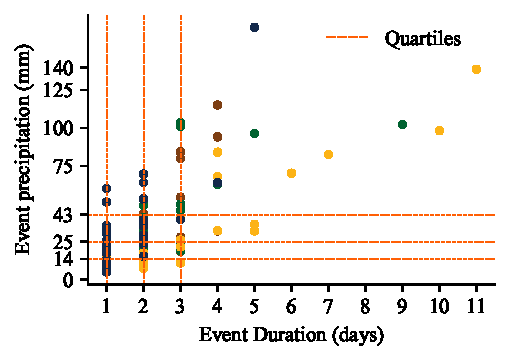
\includegraphics[width=0.7\columnwidth]{rain events}
  \caption{Event rainfall depth versus duration.}
  \label{fig:rain_events}
\end{figure}

\begin{figure}[!h] % htbp
  \centering
  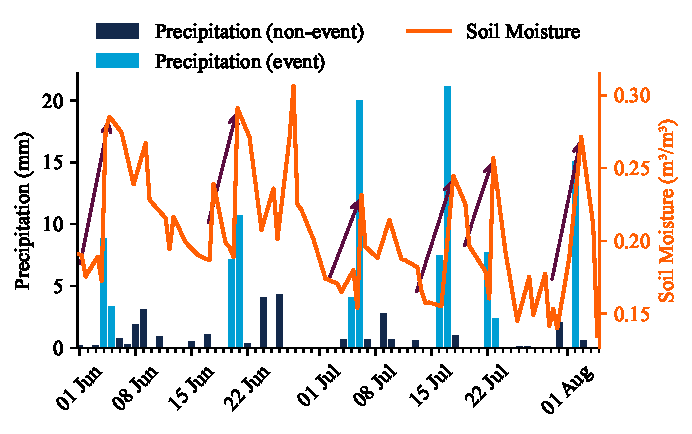
\includegraphics[width=\columnwidth]{sample events}
  \caption{Example rainfall event: daily precipitation and soil moisture response.}
  \label{fig:sample_events}
\end{figure}

\begin{figure}[!h] % htbp
  \centering
  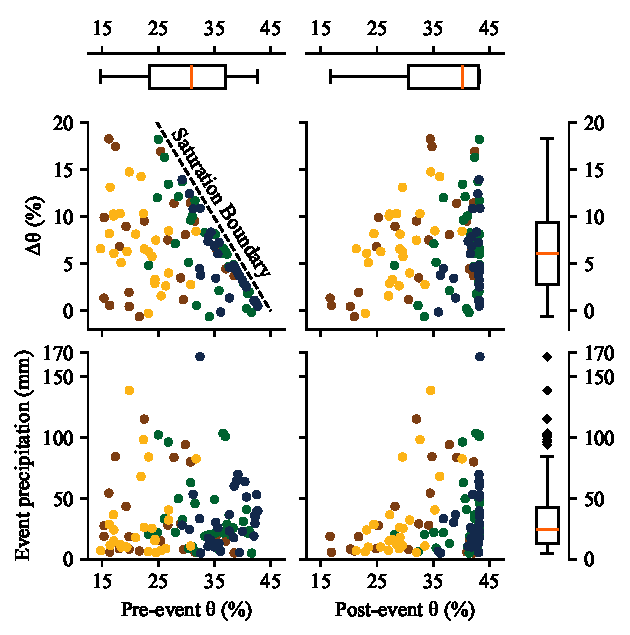
\includegraphics[width=\columnwidth]{dt events}
  \caption{Relationships among pre-event soil moisture, post-event soil moisture, event precipitation, and soil moisture change ($\Delta \theta$), with distributions of each variable shown along the axes.}
  \label{fig:dt_events}
\end{figure}

\printbibliography

\end{document}
